\documentclass[a4paper, 11pt, onecolumn]{article} 

% arara: pdflatex 
% arara: bibtex
% arara: pdflatex
% arara: pdflatex
% arara: clean: {extensions: [ aux, bbl, out, toc, blg, thm ]}

\usepackage[doi, natbibapa]{apacite}

\usepackage{enumitem}
\usepackage[english]{babel}
%if french
%\frenchbsetup{StandardLists=true}

\usepackage[T1]{fontenc}
\usepackage[utf8]{inputenc}

\usepackage{lmodern}

\let\CheckCommand\providecommand
\usepackage{microtype}
\usepackage{hyperref}
%\usepackage[pagebackref=true]{hyperref}
%\renewcommand*{\backrefalt}[4]{#1}

\usepackage{lscape}
\usepackage{graphicx}
\usepackage{amssymb,amsmath}
\usepackage{url}
\usepackage{longtable}
\usepackage{tabu}
\usepackage{siunitx}                        
%\usepackage{threeparttable} 
\usepackage{array}
\usepackage{booktabs}

%\usepackage[french]{authblk}
%\DeclareCaptionFormat{twodot}{:}
\usepackage[font=small,skip=1em]{caption}


\usepackage{setspace}
\usepackage{fullpage}
\usepackage{eso-pic}

\usepackage[explicit, clearempty]{titlesec}
\usepackage[tableposition=top]{caption}
%\usepackage{titlesec}
\usepackage[a4paper]{geometry}

\usepackage{adjustbox}
\usepackage{rotating}
\usepackage{hvfloat}
\usepackage{wrapfig}
\usepackage{tfrupee}  
%\usepackage{multicol}

\usepackage{calc}

\usepackage{lettrine}
\usepackage{oldgerm}

\usepackage{fancyhdr}
\usepackage{lipsum}  
\usepackage{lastpage}

\usepackage{changepage}

% *****************************************************************
% Annexes
% *****************************************************************
%\usepackage[title, titletoc]{appendix}
\usepackage[toc,page]{appendix}
%\renewcommand\appendixtocname{Annexes}
%\renewcommand\appendixname{Annxes}
%\renewcommand\appendixpagename{Annexes}

% *****************************************************************
% Estout related things
% *****************************************************************
\newcommand{\sym}[1]{\rlap{#1}}

\let\estinput=\input% define a new input command so that we can still flatten the document

\newcommand{\estwide}[3]{
		\vspace{.75ex}{
			\begin{tabular*}
			{\textwidth}{@{\hskip\tabcolsep\extracolsep\fill}l*{#2}{#3}}
			\toprule
			\estinput{#1}
			\bottomrule
			\addlinespace[.75ex]
			\end{tabular*}
			}
		}	

\newcommand{\estauto}[3]{
		\vspace{.75ex}{
			\begin{tabular}{l*{#2}{#3}}
			\toprule
			\estinput{#1}
			\bottomrule
			\addlinespace[.75ex]
			\end{tabular}
			}
		}

% Allow line breaks with \\ in specialcells
	\newcommand{\specialcell}[2][c]{%
	\begin{tabular}[#1]{@{}c@{}}#2\end{tabular}}

% *****************************************************************
% Custom subcaptions
% *****************************************************************
% Note/Source/Text after Tables
\newcommand{\figtext}[1]{
	\vspace{-1.9ex}
	\captionsetup{justification=justified,font=footnotesize}
	\caption*{\hspace{6pt}\hangindent=1.5em #1}
	}
\newcommand{\fignote}[1]{\figtext{\emph{Note:~}~#1}}

\newcommand{\figsource}[1]{\figtext{\emph{Source:~}~#1}}

% Add significance note with \starnote
\newcommand{\starnote}{\figtext{* p < 0.1, ** p < 0.05, *** p < 0.01. Standard errors in parentheses.}}

% *****************************************************************
% siunitx
% *****************************************************************
\usepackage{siunitx} % centering in tables
	\sisetup{
		detect-mode,
		tight-spacing		= true,
		group-digits		= false ,
		input-signs		= ,
		input-symbols		= ( ) [ ] - + *,
		input-open-uncertainty	= ,
		input-close-uncertainty	= ,
		table-align-text-post	= false
        }

% *****************************************************************
% Sources
% *****************************************************************
\newcommand{\sourcetab}[1]{\vspace{-1em} \caption*{ \textbf{Source}: {#1}} }
\newcommand{\sourcefig}[1]{\vspace{-2em} \caption*{ \textbf{Source}: {#1}} }

\addto\captionsenglish{\renewcommand{\figurename}{\textbf{Figure}}}
\addto\captionsenglish{\renewcommand{\tablename}{\textbf{Table}}}


% *****************************************************************
% Abstract
% *****************************************************************
\let\abstractname\abstracteng

% *****************************************************************
% Hypothèses
% *****************************************************************
\usepackage{ntheorem}
\theoremseparator{:}
\newtheorem{hyp}{Hypothesis}

% \makeatletter
% \newcounter{subhyp} 
% \let\savedc@hyp\c@hyp
% \newenvironment{subhyp}
 % {%
  % \setcounter{subhyp}{0}%
  % \stepcounter{hyp}%
  % \edef\saved@hyp{\thehyp}% Save the current value of hyp
  % \let\c@hyp\c@subhyp     % Now hyp is subhyp
  % \renewcommand{\thehyp}{\saved@hyp\alph{hyp}}%
 % }
 % {}
% \newcommand{\normhyp}{%
  % \let\c@hyp\savedc@hyp % revert to the old one
  % \renewcommand\thehyp{\arabic{hyp}}%
% } 
% \makeatother

% *****************************************************************
% Tableaux
% *****************************************************************
\addto\captionsfrench{\def\tablename{\textsc{Table}}}

% *****************************************************************
% Bigcenter
% *****************************************************************
%%% ----------debut de bigcenter.sty--------------
 
%%% nouvel environnement bigcenter
%%% pour centrer sur toute la page (sans overfull)
 
%\newskip\@bigflushglue \@bigflushglue = -100pt plus 1fil
 
%\def\bigcenter{\trivlist \bigcentering\item\relax}
%\def\bigcentering{\let\\\@centercr\rightskip\@bigflushglue%
%\leftskip\@bigflushglue
%\parindent\z@\parfillskip\z@skip}
%\def\endbigcenter{\endtrivlist}
 
%%% ----------fin de bigcenter.sty--------------
%%%% fin macro %%%%
\makeatletter
\newskip\@bigflushglue \@bigflushglue = -100pt plus 1fil
\def\bigcenter{\trivlist \bigcentering\item\relax}
\def\bigcentering{\let\\\@centercr\rightskip\@bigflushglue%
\leftskip\@bigflushglue
\parindent\z@\parfillskip\z@skip}
\def\endbigcenter{\endtrivlist}
\makeatother

% *****************************************************************
% Lignes de code
% *****************************************************************
\usepackage{listings}
\lstset{ 
basicstyle=\scriptsize\ttfamily,
breaklines=true,
keywordstyle=\bf \color{blue},
commentstyle=\color[gray]{0.5},
stringstyle=\color{red},
showstringspaces=false,
numbers=left,
numberstyle=\tiny \bf \color{blue},
stepnumber=1,
numbersep=10pt,
firstnumber=1,
numberfirstline=true,
frame=leftline,
xleftmargin=0.5cm
}
 
% *****************************************************************
% Auteurs en bleu
% *****************************************************************
%\renewcommand{\citep}[1]{\textcolor{teal}{\citep{#1}}}
%\renewcommand{\cite}[1]{\textcolor{teal}{\cite{#1}}}
\usepackage{xcolor}
\usepackage{colortbl}

\hypersetup{colorlinks,linkcolor={red},citecolor={teal},urlcolor={blue}}
%\newcommand{\ypenser}[1]{\textcolor[purple]{#1}}
\newcommand{\ypenser}[1]{\textbf{\color{purple}--#1--}}

% *****************************************************************
% Mail
% *****************************************************************
\newcommand{\email}[1]{\href{mailto:#1}{\nolinkurl{#1}}}

% *****************************************************************
% Résumé et mots clés
% *****************************************************************
 \newenvironment{resab}[1]
{\begin{adjustwidth}{0cm}{0cm} \hangafter =1\par
    {\normalsize\bfseries #1\ \\ }\normalsize}
{\end{adjustwidth}\medskip}

 \newenvironment{keywords}
{\begin{adjustwidth}{0cm}{0cm} \hangafter =1\par
    {\normalsize\itshape Keywords:}~\normalsize}
{\end{adjustwidth}\medskip}

 \newenvironment{jelcodes}
{\begin{adjustwidth}{0cm}{0cm} \hangafter =1\par
    {\normalsize\itshape JEL Codes:}~\normalsize}
{\end{adjustwidth}\medskip}

% *****************************************************************
% Poete
% *****************************************************************
\newcommand{\attrib}[1]{%
\nopagebreak{\raggedleft\footnotesize #1\par}}

% *****************************************************************
% Stata
% *****************************************************************
\newcommand{\Stata}{%
\textsc{Stata$^{\mbox{\scriptsize{\textregistered}}}$}
}

% *****************************************************************
% Encadré
% *****************************************************************
\usepackage{tikz}

% Thick
\def\checkmark{\tikz\fill[scale=0.4](0,.35) -- (.25,0) -- (1,.7) -- (.25,.15) -- cycle;} 

\newcommand{\titlebox}[2]{%
\tikzstyle{titlebox}=[rectangle,inner sep=10pt,inner ysep=10pt,draw]%
\tikzstyle{title}=[fill=white]%
%
\bigskip\noindent\begin{tikzpicture}
\node[titlebox] (box){%
    \begin{minipage}{0.94\textwidth}
#2
    \end{minipage}
};
%\draw (box.north west)--(box.north east);
\node[title] at (box.north) {#1};
\end{tikzpicture}\bigskip%
}

% *****************************************************************
% Changer la forme des titres
% *****************************************************************
 %\titleformat{\section}[block]			%section + style prédéfini par l'extension (block = 1 ligne)
 %{\sffamily\bfseries\LARGE\titlerule[1pt]}						%format pour le titre + label
 %{\sffamily\bfseries\LARGE}						%format pour le titre + label
 %{\sffamily\bfseries\LARGE\arabic{section}}		%format que pour le label
 %{0.5cm}								%espace qui sépare le label du titre
 %{#1}									%description du style pour le titre uniquement
 %\titlespacing{\section}				%section
 %{0cm}									%espace à gauche du titre
 %{3em}									%espace verticale AVANT le titre
 %{1em}									%espace verticale APRES le titre
 %%{0cm} 								%espace à droite du titre: mettre la même valeur que gauche pour un peu centrer

 %\titleformat{\subsection}{\sffamily\bfseries\Large}{\thesubsection}{0.4cm}{#1}
 %\titlespacing{\subsection}
 %{1cm}
 %{2em}
 %{1ex}

 %\titleformat{\subsubsection}{\sffamily\bfseries\large}{\thesubsubsection}{0.4cm}{#1}
 %\titlespacing{\subsubsection}
 %{2cm}
 %{2em}
 %{1ex}

% *****************************************************************
% Style de la date
% *****************************************************************
%\def\mydate{\leavevmode\hbox{\the\year-\twodigits\month}}
\def\mydate{\leavevmode\hbox{\the\month-\twodigits\year}}
\def\twodigits#1{\ifnum#1<10 0\fi\the#1}

% *****************************************************************
% En tête
% *****************************************************************

% Pour les numéros de pages
%\pagestyle{fancy}

% Si tu veux mettre les numéros genre: 1/22
% Il faut que tu écrives
% "\thepage/\pageref{LastPage}"
% Sans les " " dans les lignes en bas: \fancyhead[...

% Ca c'est pour enlever la barre horizontale sous l'entête
% Pour la laisser tu mets "1pt" au lieu de 0
\renewcommand{\headrulewidth}{0pt}
\renewcommand{\footrulewidth}{0pt}

% fancyhead pour l'entête
% fancyfoot pour le pied de page
% L=left; R=right; C=center
%\fancyhead[L]{\textcolor{gray}{\textsf{\textit{Revue de la littérature autour du mariage: le cas de l'Inde}}}}
%\fancyhead[R]{\textcolor{gray}{\textsf{Natal, A. (\mydate)}}}
%\fancyfoot[C]{\thepage}
%updmap.exe --admin

%\lhead{\textcolor{gray}{\textsf{\textit{Revue de la littérature autour du mariage: le cas de l'Inde}}}}
%\rhead{\textcolor{gray}{\textsf{Natal, A. (\mydate)}}}
\cfoot{\thepage}

% *****************************************************************
% Jatis
% *****************************************************************
\newcommand{\jati}[1]{\textit{j\={a}ti{#1}}}

% *****************************************************************
% Enlever le titre Table des matières
% *****************************************************************
%\makeatletter
%\renewcommand\tableofcontents{%
%    \@starttoc{toc}%
%}
%\makeatother

% *****************************************************************
% À développer
% *****************************************************************
\newcommand\dev[1]{\textbf{\textcolor{red}{#1}}}

% *****************************************************************
% Fonts
% *****************************************************************
%\usepackage{tgbonum}
\usepackage{kpfonts}

% *****************************************************************
% Taille des tableaux
% *****************************************************************
\let\oldtabular=\tabular
\def\tabular{\small\oldtabular}
%\def\tabular{\normalsize\oldtabular}

% *****************************************************************
% Style de la biblio
% *****************************************************************
\bibliographystyle{apacite}

% *****************************************************************
% Numérotation
% *****************************************************************
%\usepackage{lineno}

% *****************************************************************
% Titre et page de garde
% *****************************************************************
\usepackage{titling}
\setlength{\droptitle}{-2cm}
\pretitle{\begin{center}\fontsize{24pt}{10pt}\selectfont\bfseries}
\posttitle{\par\end{center}\vskip 1ex}
\preauthor{\begin{center}
    \large \lineskip 0.5em}
\postauthor{\par\end{center}}
%\thanksheadextra{1,}{}
\thanksheadextra{}{}
\setlength\thanksmarkwidth{.5em}
\setlength\thanksmargin{-\thanksmarkwidth}


% *****************************************************************
% Symboles
% *****************************************************************

\def\@fnsymbol#1{\ensuremath{\ifcase#1\or *\or \dagger\or \ddagger\or
   \mathsection\or \mathparagraph\or \|\or **\or \dagger\dagger
   \or \ddagger\ddagger \else\@ctrerr\fi}}
   
\makeatletter
\newcommand{\ssymbol}[1]{^{\@fnsymbol{#1}}}
\makeatother
   
   
   
% *****************************************************************
% Makecell
% *****************************************************************
\usepackage{makecell}
\newcommand\Tablenote[2]{\multicolumn{#1}{l}{\makecell[l]{\textit{Note:}~#2}}}


   

%\usepackage{fonttable}

\usepackage{import}

\usepackage[
singlelinecheck=false % <-- important
]{caption}

\usepackage{upgreek}

\newcommand{\ie}{\textit{i.e.}}

% \renewcommand*\thetable{\Alph{section}.\arabic{table}}
% \renewcommand*\thefigure{\Alph{section}.\arabic{figure}}


% *****************************************************************
% Interlignes et marges
% *****************************************************************
\setstretch{1}
\geometry{%
left=2.5cm,
right=2.5cm,
top=2.5cm,
bottom=2.5cm,
%includefoot,
%headsep=1cm,
%footskip=1cm
}%

% *****************************************************************
% Page de garde
% *****************************************************************
\title{Indebtedness in Rural India: The Contribution of Cognitive Skills and Personality Traits}
\author{Arnaud Natal\thanks{Univ. Bordeaux, CNRS, GREThA, UMR 5113, F-33600 \textsc{Pessac, France} - \email{arnaud.natal@u-bordeaux.fr}} ~ \& Christophe J. Nordman\thanks{IRD, UMR LEDa-DIAL, IFP - \email{nordman@dial.prd}} }
\date{\today}
\renewcommand\maketitlehookc{%
  \begin{center}
    %\textsuperscript{1}{\small Université de Bordeaux}
    \textsuperscript{}{\normalsize Preliminary draft}
  \end{center}}

% ******************************************************************
\begin{document}
\maketitle

\hrule 
\vspace{0.3cm}

\begin{resab}{Abstract}

\end{resab}

\begin{motkey}{Keywords}
Gender, caste, 
\end{motkey}


\hrule
%\linenumbers

% ******************************
\section{Introduction}
% \addcontentsline{toc}{section}{Introduction}
\label{Introduction}
% ******************************

Nouvelle organisation de la revue, sûrement meilleure
\begin{itemize}
\item Depuis quelques années, les institutions s'intéressent de plus en plus au rôle de la personnalité et des compétences cognitives.
Faire un paragraphe complet là-dessus.
\item Puis s'amener à se demander ce que c'est et les travaux académiques en économie.
Définition simple du Big-5, avec la revue skills \& outcomes.
\item D'accord, les sujets classiques en éco sont traités et depuis peu quelques travaux regarde ça sur l'endettement des ménages et ils font bien car c'est super important comme sujet: 
Pourquoi c'est important ? 
Literature on subject?
\item Argument 1 sur la pertinence: Très peu de travaux s'intéressent aux pays en développement alors que c'est là-bas que le sujet est encore plus intéressant par rapport aux différentes politiques:
Inclusion financière = bancariser les plus pauvres 
Lutte contre la pauvreté = 
\item Argument 2 sur la pertinence: Et notamment en Inde, où l'endettement des ménages est colossal:
literature
\item Argument 3 sur la pertinence: Avec énormément d'inégalités:
literature
\item Argument 4 sur la pertinence: Ces inégalités sont tellement fortes qu'elles brident les individus, elles les renferment dans le genre et la caste:
literature sur les aspirations
\item Conclusion:
Après avoir regardé le lien entre personnalité et dette (arguments 1 et 2), on va chercher à voir si dans les carcans, des individus arrivent à se différencier par leurs personnalité en matière de dette (arguments 3 et 4). 

\end{itemize}


Despite the recent economic growth\footnote{World Bank Data -- \url{https://data.worldbank.org/indicator/NY.GDP.MKTP.KD?locations=IN}. Accessed June 21, 2021.} and the improvement in education and health, social disparities subsist in India, especially through the caste system and gender.
Historically, caste --or \jati, represent an hierarchical and endogamous group of individuals based on occupation.
With gender, it represent the major sources of inequality in terms of education \citep{Munshi2006, Hasan2006, Saha2013}, labour \citep{Madheswaran2007, Mohanty2006, Das2012}, wealth and poverty \citep{Borooah2005b, Zacharias2011, Deshpande2000, EsteveVolart2004} or marriage \citep{Banerjee2009, Chacko2003}.

		% ******************************
		\subsubsection{Conditioned individuals through caste and gender with aspirations}
		% ******************************
More recently, several works highlight disparities between \jati ~and gender in terms of aspirations.
\cite{Mukherjee2017} show that ``gender and caste primes can significantly affect long run aspirations and beliefs''. 
\cite{Alvi2019} use priming\footnote{Priming, in cognitive psychology, is ``the effect in which recent experience of a stimulus facilitates or inhibits later processing of the same or a similar stimulus.'' -- \url{https://dictionary.apa.org/priming}. Accessed June 21, 2021.} to study the effect of identity salience on aspirations.
They find that ``when women are primed on gender, they exhibit higher aspirations for their daughters [and] low-case  women primed on caste are more aspirational for their daughters''.
Finally, \cite{Sarkar2020} show that caste and gender work as double jeopardy instead of intersectionality for aspirations.
Indeed, ``the most socially disadvantaged groups -- Scheduled Tribe (ST) and Scheduled Caste (SC) -- have significantly lower income aspiration when compared to Other Backward Class (OBC) and Other Caste (OC) partiipants'' [and] [f]emale participants also have significantlty lower aspiration than their male counterparts''.
Moreover, SC/ST female participants have lower income aspiration levels compared to other groups.
Thus, beyond being a source of inequality, \jati and gender seems to deeply impact individuals by conditioning them.
More than an fregmentation and more than sources of dispartities, caste and gender seems to deeply impact social identities of individuals in India.
Indeed, it seems to conditionned individuals, it is part of their identity that affect action deep inside them as determine their aspirations.
In this context it appears important to analyse the role of personality traits \& cognitive skills on debt in take into account the deepness of this social identity.
% For that, we use sub-sampling technic and we analyse the role of cognitive skills into this specific social identity.
% We create four group of individual : female dalits (i); male dalits (ii); female middle and upper class (iii); male middle and upper class (iv). 
% Three groups on four appears to be socially disadvantaged and one support the double jeopardy (DJ) thanks to \cite{Sarkar2020} (see Table \ref{tab:subsampling}).


Aspirations limitée par notre caste et notre sexe.



	% ******************************
	\subsection{Debt}
	% ******************************
	
Less work try to understand this disparities in terms of debt while it is an important research topic.
		
		% ******************************
		\subsubsection{Incidence of debt with disparities}
		% ******************************

The Indian context is unique in terms of household finance \citep{Badarinza2016b}.

\% HH concerned and amount with \cite{NSSO2014}
The largest part of households debt is informal in rural India \citep{Badarinza2016b}.
\begin{itemize}
\item car les terres et les maisons s'héritent : \citep{Badarinza2016b} avancent que cela peut provenir de la « prédominance des ménages multigénérationnels, dans lesquels les terres et les propriétés résidentielles constituent une part importante des legs » donc pas beaucoup besoin d'emprunt formel. 4\% des ménages dont le chef a moins de 35 ans ont un prêt hypothécaire ce qui est nettement inférieur à la situation des autres pays émergents comme la Chine \citep{Badarinza2016b}.
\item Pénétration bancaire très hétérogène : \citep{Badarinza2016b} et \citep{Burgess2005} : les États ayant un taux de pénétration bancaire élevé sont ceux où les ménages sont les moins dépendants de l’endettement non institutionnel.
\end{itemize}
%D'après \citep{Badarinza2016b}, la proba de contracter une dette informelle se réduit avec le niveau d'éducation: [l]es ménages dont au moins un membre a fait des études supérieures ou des études de troisième cycle ont une dette hypothécaire supérieure de 15,1\% par rapport au groupe des personnes peu instruites et une part de dette non institutionnelle inférieure de 28,7\%.

Paysage financier de \cite{Guerin2012a} for informal debt and reasons of debt: beaucoup de cérémonies, beaucoup de survie quotidienne.

%Determinants?  \citep{Datta2018, Pandey2016}

\dev{OK, on voit que beaucoup de monde est concernés, avec tel montant, tel type de dette et telle raison, mais many disparities.}
Disparities 
\begin{itemize}
\item \cite{Guerin2013a} show that caste affect borrowing strategies as amount, type and source of debt in rural India.
Moreover, they show that debt is a ``social transaction which inscribes debtors and creditors into local system of hierarchies''.
\item \cite{Reboul2021} find an interest in the gender perspective.
\item Debt bondage for dalits \citep{Guerin2020a}
\item The case of microfinance for womens \citep{Guerin2020b}
\item  Castes, sex, moc, etc.  \citep{Guerin2012a} \citep{Guerin2013a} \citep{Guerin2014} \citep{Reboul2021}
\end{itemize}

%Failures for repayment, violence, overindebtedness, microcredit \citep{Sedai2021}


		% ******************************
		\subsubsection{Individual debt and public policies}
		% ******************************

\begin{itemize}
\item Financial inclusion : more and more HH are financial included \citep{Badarinza2019}, especially in India \citep{Chakravartya2013}. \dev{Literature Isabelle}
\item Secondly, on a vue que quasi tout le monde est concernés par la dette et especially to consume which is an determinants of global wealth (expenditures approach of GDP).
In India, the households and non-profit institutions serving households (NPISHs) final consumption expenditure represent 60.29\% of GDP\footnote{World Bank Data -- \url{https://data.worldbank.org/indicator/NE.CON.PRVT.ZS?locations=IN}. Accessed January 22, 2021.}.
\item Household finance has faced a renewed interest since a decade \citep{Guiso2013}.
Indeed, household are more implicated in financial decision such as privatization of retirement pension, liberalization of loan market, increase in credit purchase, which are more complicated because of financial innovation\footnote{For a comprehensive review on the subject, see \cite{Tufano2003}.}.
%Household finance (or consumer finance for researchers in business sciences) refer to the way that ``households use financial instruments to attain their objectives'' \citep{Campbell2006}.
%More precisely\footnote{For a comprehensive review on household finance, see \cite{Tufano2009} for whom household finance is ``the study of how institutions provide goods and services to satisfy the financial functions of households, how consumers make financial decisions, and how government action affects the provision of financial services'', \cite{Guiso2013}, or \cite{Xiao2020}.}  its a ``research field to study how financial institutions provide products and services to meet financial needs of consumers, how consumers make financial decisions, how government agencies regulate financial institutions and protect financial consumers and how science and technology help optimize the efficiency of consumer finance markets and improve social welfare'' \citep{Xiao2020}.
\end{itemize}





		% ******************************
		\subsubsection{Debt is not just money, it is social link}
		% ******************************
\begin{itemize}
\item Question de la confiance très présente dans la dette :
\cite{Guerin2014a} Households’ creditworthiness is above all a matter of trust (nambikai), the term used locally
when people refer to their ability to access credit. The fabric of trust covers many aspects that
far exceed good credit history and repayment behaviour, and relates to every aspect of the
borrowers’ reputation. Creditworthiness is rarely assessed on the individual level, and often
incorporates the reputation and morality of the whole family or even lineage (Harriss-White
and Colatei 2004). Lenders often state that they take two levels into account. One relates to
family and lineage (taradaram), namely the family’s history, its “ethical” background and
“morality”. The second level is individual (daram), relating very broadly to the “quality” of a
person. It is therefore perfectly rational that the poor attach an equal importance to their
reputation.

“Behavior” also matters. As previously discussed, low castes are often seen as risky
borrowers. Irrespective of caste, bad habits such as laziness, alcoholism and gambling are
considered as indicators of poor repayment potential. As discussed above, respect and deference are also highly valued. Potential borrowers should equally show respect to their
lenders and at times to its community.
Giving money is a matter of respect. I respect them, they should respect me. How could I give them
money if they talk badly about me? (Rajagopalan, Reddiar [FC], landowner and lender).
If you don’t want credit from a particular community, then you can talk about them to others; otherwise
you should not criticize. It might spoil creditworthiness. We should talk respectfully about these people,
this is the only way to get creditworthiness (Gundusammy, Goundar (MBC), agriculture coolie and
marginal farmer).

\item Rapport de force
\cite{Guerin2014}

\citep{Guerin2020a}
inseparable from an overall set of interdependencies, protection and social differentiation

\item Social and moral experience
imbued with subjectivities, felt-obligations and also aspirations

\item Prestige sociale
\cite{Guerin2014a}
To understand debt practices, motivations and rationales, however, it is necessary to examine
how the poor perceive and experience debt. It also requires taking into account the diversity
of debt meanings and debt relationships. Of those in extremely vulnerable financial situations,
very few consider themselves as over-indebted. The contrast between exogenous
categorisations and local subjectivities is striking. One could of course argue that the poor
suffer from “false consciousness”, in the sense that they are not even able to assess their own
exploitation. Our explanation is different: we argue that the poor have their own “frameworks
of calculations” (Villarreal 2009; this volume) and debt hierarchies (Shipton 2007). Such
phenomena transcend questions of material or self-centred motivations and reflect issues of
status, honour, power, and individual and group identity. This is our second argument:
individuals engage multiple criteria to establish debt hierarchies and to evaluate debt burdens.
Though financial criteria certainly matter, the social meaning of debt is equally, or more
valued. While some debts are dishonoring, others are not. This depends upon the social
relation between the debtor and the creditor and their respective status. Caste, class, kin and
gender relationships are instrumental here.

\cite{Guerin2014}
Firstly, the social meaning of debt clearly matters. Debt is a marker of social hierarchy in
kinship groups, the neighborhood and community alike. People try to avoid debts degrading
to their status, or at least try to pay back these debts first.

\end{itemize}


\cite{Guerin2014a} : What is however clear is that over-indebtedness as a concept has little meaning to the poor.
Financial indicators are certainly useful (and will be used here) to quantify the cost of debt.









	% ******************************
	\subsection{Cognitive skills}
	% ******************************

		% ******************************
		\subsubsection{Accroche avec les insitutions et les défintions}
		% ******************************

% In psychology, it's well known that individuals are differents each others.
% Many studies in economics and more recently instutions\footnote{World Bank} sought to analyse this.	
	
% Cognitive skills can be defined as a ``term that refers to mental processes involved in the acquisition of knowledge, manipulation of information, and reasoning [that] include the domains of perception, memory, learning, attention, decision making, and language abilities'' \citep{Kiely2014}.

% While ``personality is the dynamic organization within the individual of those psychophysical systems that determine his characteristics behavior and thought'' \citep{Allport1961}.
% Among the theories of personality, the traits can be define as thought, emotion and habitual patterns of behavior \citep{Kassin2003}.
The Big-Five model --or Five Factor model (FFM)-- constitute the main personality trait taxonomy.
Based on \cite{Goldberg1981} and \cite{McCrae1987} works, this taxonomy identify five dimensions of personality from factor analysis [on specific questionnaires]: neuroticism (i), \ie~the capacity to experience negative emotions (anxiety, anger, depression, etc); extraversion (ii), \ie~the energy, the capacity to experience positive emotions, the tendency to seek stimulation and company from others; openness to experience (iii), \ie~``one’s capacity to be creative and unstructured versus one’s tendency to need structure and clarity'' \citep{Piedmont2014}; agreeableness (iv), \ie~``perceptions of others that are caring, compassionate, and altruistic versus manipulative, self-serving, and antagonistic'' \citep{Piedmont2014}; conscientiousness (v), \ie~the capacity to display self-discipline, act dutifully, and strive for achievement against measures or outside expectations.	
	
%\footnote{Themselves inspired by the work of \cite{Cattell1943, Cattell1947} and \cite{Norman1963}.}
	
		% ******************************
		\subsubsection{Cognitive skills in economics}
		% ******************************
	
Since a decade, intrinsic differenciation of individual through cognitive skills and personality traits is increasingly examining by researchers and institutions. 
\cite{Almlund2011} for comprehensive review, but explain output on labor, education, crime.
%Décollage au début des années 2000\footnote{Préciser en footnote qu'il y a eu \cite{Bowles1976} avant qui a regardé les earnings, mais vraiment très peu de travaux.} avec le marché du travail est notamment:
Labor market:
\begin{itemize}
\item[1] les différences de rémunérations \citep{Bowles2001} \citep{Heckman2006}  \citep{Cawley2001}
\item[2] performance au travail : la consciensiocité est le trait qui prédit le mieux la performance au travail de facon générale: \citep{Nyhus2005} \citep{Salgado1997} \citep{Hogan2003} \citep{Barrick1991}
\item[3] type de travail : À la différence du quotient intellectuel (Q.I.), ce trait de personnalité ne varie pas avec la complexité du travail effectué, laissant penser que la conscienciosité concerne un plus large éventail d’emplois. En effet, les professeurs, les scientifiques et les cadres supérieurs ont en général de meilleurs résultats en matière de compétences cognitives par rapport à des travailleurs non qualifiés \citep{Schmidt2004} \citep{Almlund2011} \citep{Barrick1991}. + \citep{CobbClark2011} trouvent que le degré d’agréabilité a une relation négative avec la probabilité d’être un manager et d’être un professionnel des affaires (business professional).
\end{itemize}

Education: On regarde aussi l'éducation où \cite{Almlund2011} : Avant tout, les auteurs constatent que parmi les cinq (5) traits du Big Five, la conscienciosité et le névrosisme prédisent bien un grand nombre d’outcomes, notamment ceux en rapport avec l’éducation (la conscienciosité explique assez bien l’attainment et achievement à l’école). L’ouverture à l’expérience prédit, elle, assez bien la course difficulty selected et l’attendance.

Santé: Lorsque les variables expliquées sont en rapport avec la santé, la conscienciosité est le meilleur prédicateur pour la longévité de vie (plus que l’intelligence et le background) \citep{Almlund2011}

Crime: Enfin, lorsque les auteurs s’intéressent à la littérature sur la criminalité, ces derniers relèvent que la conscienciosité et l’agréabilité sont d’importants prédicteurs de la criminalité \citep{Almlund2011} 




		% ******************************
		\subsubsection{Skills and debt}
		% ******************************

%Even if the study of cognitive skills and personality traits have started to attract the attention of labor-economist \citep{Almlund2011}, 

Few researcher have been interested in the relationship with household finances while ``it is apparent that personality traits may influence financial decision-making at the individual and household level'' \citep{Brown2014}.

Mais quelques travaux sur financial literacy qui lie un peu les la dette et les skills \citep{Hastings2013} \citep{Varum2014} \citep{Pinjisakikool2017} \citep{Gaurav2012} \citep{Hastings2013} 

Les premiers travaux qui lie skills et hh finance ont moins de 10 ans et s'intéressent principalement à:
\begin{itemize}
\item[1] décision d'investissement, financial distress : \citep{Nga2013} \citep{Pinjisakikool2017b} \citep{Bucciol2017} \citep{Agarwal2013} \citep{Parise2019}
\item[2] épargne  : \citep{CobbClark2016} \citep{Gerhard2018}
\item[3] dette : \citep{Forlicz2019} \citep{Silva2018} \citep{Brown2014}
\end{itemize}









	% ******************************
	\subsection{Topic relevance}
	% ******************************
%Microfinance a ciblé les femmes car plus souple et plus facile à ménacer = dimension psychologique très importante? 



C'est d'autant plus intéressant que la dette est omniprésente \cite{Guerin2013, Guerin2020}

Try to capture the role of cognitive skills and personality traits thus allows to better understand the determinants of indebtedness in India, which is an important vector of wealth through consumption. 
%Consumption expenses represent almost a third of loans in 2010 and 2016-17 --this is the most common loan reason-- and the average amount of one loan is 9,920 INR in 2010 and 24,780 INR in 2016-17.


\dev{Est-ce qu'il y a un lien entre compétences cognitives et endettement ?}
\dev{Plus particulierement, est-ce qu'à l'intérieur des carcans, des individus se différencient par leurs compétences cognitives ?}










\newpage
% ******************************
\section{Data and methodology}
% ******************************


	% ******************************
	\subsection{Data}
	% ******************************

Our empirical analysis is based on the NEEMSIS-1 \& NEEMSIS-2 (Networks, Employment, dEbt, Mobilities and Skills in India Survey) surveys carried out respectively in 2016-17, and 2020-21 \citep{NEEMSISreport, NEEMSIS2017}.
This survey was the second and third waves of a longitudinal data collection project start in 2010 with RUME (RUral Microfinance and Employment survey) project in ten villages of Tamil Nadu.
Located in the Cuddalore and Villupuram districts, a mostly agricultural area, economies benefits from the proximity of two large industrial towns (Neyveli and Cuddalore) and a regional business center (Panruti).

RUME randomly selected 405 households using stratified sample framework based on three dimensions: proximity to small towns (Panruti, Villupuram and Cuddalore), an agro-ecological criterion, and caste affiliation.
Thus, half of villages are irrigated (the other half have dry lands) and within villages, half of the sample was selected from the mostly upper and middle caste part of the village (Ur) while the other half from the Colony part, where dalits (the ex-untouchables)  mainly live. 
NEEMSIS1 recovered 388 households (4.19\% attrition rate) and randomly selected 104 news households (for a total of 492 households) from these 10 villages, based on the same method. 
%Given that some households had migrated elsewhere between the 2010 and 2016-17 sampling periods (13\% of the recovered households).
NEEMSIS2 recovered 485 households (1.42\% attrition rate) from 2016-17 and recovered 10 households from 2010 that were not recovered in 2016-17.
Moreover, 100 news households were randomly selected (for a total of 595 households).

%While RUME survey focus on employment, migration and remittances, financial practices (such as loans, savings, lending practices, gold), agriculture, consumption and housing at household level, a new individual questionnaire have been added to NEEMSIS.
In NEEMSIS1 \& NEEMSIS2, two household members, called ``ego 1'' (mostly household questionnaire respondent) and ``ego 2'' (one younger household member randomly selected on a criterion of age), are directly addressed individual questionnaires that provide for instance a range of information on cognitive skills and personality traits.

NEEMSIS's surveys stands out from other Indian data sources such as the All India Debt and Investment Survey (AIDIS), as it has the rare and valuable advantage of recording debt at the individual level (identifying the person who went to the lender and borrowed in her own name).

Concerning the reliability, the great expertise of the team\footnote{Some members of the research team are present since more than twenty-year on the region for numerous quantitative and qualitative surveys.}, helped to formulate questions appropriately.
This for instance involved using particular terms that are less degrading than the generic term ``debt'' lists of the main local lenders, and asking indirect questions.
As stated by \cite{Reboul2021} (same data sets) ``[i]mproved data accuracy is for example reflected by an incidence of indebtedness found higher than in the estimates of the nation-wide AIDIS: 99\% of households are in debt in our case study, as opposed to 30\% in rural Tamil Nadu in 2012 according to the AIDIS \citep{NSSO2014}.'' 

Moreover, the moderate magnitude of the survey, compared to nationally representative datasets, ensures the high quality of the data and the tablet-based mode of data collection improved data quality in including constraints on answers to prevent inconsistencies. 

Our final sample consists of 473 households and 835 egos because in 2016-17, two households does not have egos; and for 10 households all egos have changed between 2016-17 and 2020-21 (see Appendix \ref{app:data}).







	% ******************************
	\subsection{Construction of personality traits \& cognitive skills variables }
	% ******************************

As stated earlier, our survey allow us to construct Big-5 personality traits.
On the basis of 35 questions relatives to Big-5 taxonomy, we averaged answers --based on a  Likert scale from 1-``Almost Never'' to 5-``Almost always'', that belong to a determined trait after correcting for acquiescence bias\footnote{Acquiescence bias represent the ``tendency for survey respondents to agree with statements regardless of their content'' \citep{Lavrakas2008}.} (see Appendix \ref{section:efa_big5}).
The resulting mean represent the score on each traits.

\citeauthor{McDonald1999}'s $\upomega$\footnote{Literature on internal consistency estimators increasingly agrees that \citeauthor{Cronbach1951}'s $\upalpha$ --the most wide used estimator, is maybe not very efficient \citep{Bourque2019, TrizanoHermosilla2016}.}, a measure of internal consistency, are mostly satisfactory: 0.81 for openness; 0.86 for conscientiousness; 0.59 for extraversion; 0.60 for agreeableness and 0.80 for emotional stability.
%It is for corrected one
%For raw: 0.85 for OP; 0.84 for CO; 0.71 for EX; 0.43 for AG; 0.64 for ES
%0.60 (agreeableness), 0.61 (extraversion), 0.68 (grit), 0.77 (emotional stability), 0.78 (openness to experience), and 0.85 (conscientiousness)

Cognitive skills include three score variables: literacy, numeracy, Raven\footnote{Raven test is ``a nonverbal test of mental ability consisting of abstract designs, each of which is missing one part. The participant chooses the missing component from several alternatives to complete each design.'' -- \url{https://dictionary.apa.org/ravens-progressive-matrices}. Accessed January 27, 2021.}.
These scores are construct in adding up the correct answers of a set of four questions for literacy and numeracy test and 36 for Raven.

\paragraph{Exogeneity}
The exogeneity of personality traits is well assume because of stability over time while there is no consensus in psychology \citep{Ardelt2000}.

According to \cite{Costa1997, McCrae2000} it remains stable, in part, because it is a genetic predisposition that, by definition, cannot be changed over life.
Economist follow this path and the majority of then assume stability over time after the age of 25 and other verify this stability \citep{CobbClark2011}. 

This stability refutes sociological and psychological literature which interesting in the influence of childhood and adulthood socialization on personality \citep{Mortimer1978, Moen1995}.
Following this path, \cite{Ardelt2000} state that ``personality can change over the course of a person's life, particularly if age at first measurement is low or over 50, if the retest interval is large, if individual personality aspects rather than the overall personality are considered, and if personality aspects other than the big five NEO traits are assessed.''
%\footnote{See \cite{Ardelt2000} for comprehensive review on critics of stability.}

% \citep{Ardelt2000}
% First, ideally, it would be most promising to study personality before and after unexpected, drastic changes in people's social environments, particularly those which conflict with their existing personality dispositions (Caspi 1993; Stokes et al. 1989).
% Unemployment, a terminal illness, incarceration, natural disasters, or sudden political or economic upheaval tend to force individuals to adapt to an environment that they did not select and that may be difficult to shape and transform in accordance with their personality characteristics.
% Under those circumstances, successful adaptation indeed may require a change in the individual's personality. 
% Unfortunately it is generally not known when these unexpected changes in the social environment will occur; therefore studies of this kind will require a large budget to follow a diverse segment of society over a long period.

Our data allow us to examine stability over time of Big-5 personality traits for 835 individuals of rural India.
Calculating variation rate between 2016-17 and 2020-21 of each traits, results show a stability for minor part of the population (see Table \ref{fig:stab} of Appendix \ref{section:stab_big5}).

Thus, in order to limit endogeneity --through reverse causality, we investigate the role of personality traits and cognitive skills (and all others independents variables) in 2016-17 on 2020-21 debt.



\paragraph{Factor analysis}
As warned by \cite{Laajaj2019}, the Big-Five taxonomy is limited in developing countries for several reasons: the enumerator-respondent interactions (i) in face-to-face survey can induce a bias; the low education levels (ii) can make questions more difficult to understand and can induce a systematic response patterns, especially the acquiescence bias (iii).

The very good knownledge of the field allow us to collect data of high quality and avoid a bias due to misunderstanding of questions.
Moreover, we implement our own factor analysis of the 41 questions by principal component with promax rotation.
To avoid a bias in factor analysis, we do not corrected for acquiescence bias.
In our dataset, acquiesence bias is measure with a set of inverse questions that are supposed to measure the same aspect of personality. 
This assumption is true only in the context of Big-5 model. 
In another context, the questions can, perhaps, have a different meaning.

The resulting factors are relatively similar to the Big-5 personality traits (see Table \ref{tab:corrbig5efa}) with satisfactory \citeauthor{McDonald1999}'s $\upomega$: Factor 1 as Extraversion-Openness ($\upomega=0.91)$; Factor 2 as Conscientiousness ($\upomega=0.87)$; Factor 3 as Emotional stability-Conscientiousness ($\upomega=0.76)$; Factor 4 as Emotional stability ($\upomega=0.81)$ and Factor 5 as Agreeableness ($\upomega=0.64)$.

\paragraph{Life-cycle effects}
To mitigate against the potential problem of life-cycle events --that might induce endogeneity through measurement error, we run univariate OLS regression with cognitive skills and personality traits as endogenous variables and age as exogenous variable (see Appendix \ref{section:efa_big5}).
We standardised the resulting residuals and use it as cognitive and personality measures net of life cycle influences \citep{Nyhus2005, Brown2014}. 

% $S_k$ (where $k=1, 2, 3$ for raven, literacy, numeracy)
% $P_k$ (where $k=1,...,10$ for Big-5 personality traits and factor analysis traits)
% $A$
% $S_k=\upphi A+\upvarepsilon_j$ (eq. i) and $P_k=\upphi A+\upvarepsilon_j$ (eq. ii)
% residual $\hat{\upvarepsilon_j}$ 


\subimport{INPUT}{corrBig5EFA.tex}



	% ******************************
	\subsection{Indebtedness measures}
	% ******************************

Before exploring the role of cognitive skills and personality traits, it is necessary to discuss debt and over-indebtedness measures.
There is no consensus in the literature but three approaches are often retained \citep{Betti2007, Ferreira2000}.
Objective measures focus on the ability (or inability) to service or repay debts.
Typically, it is the debt to income ratio, debt to asset ratio, debt service ratio.
Over-indebtedness occurs when a certain threshold is exceeded.
Although this is the most widely used measure, it under-estimate the burden of debt in ousting personal feeling and sacrifice associated with debt and over-indebtedness \citep{Betti2007}.
 
Subjectives measure assume that ``individual households are the best judges of their own net debt/wealth position'' \citep{Betti2007}.
The robustness of the results are based on the degree of honesty and literacy of individuals that can make it, sometimes, less reliable \citep{Betti2007, DAlessio2013}.
As stated by \cite{Rinaldi2006} and \cite{Keese2012}, in general, objective measures align quite well with subjective measures at the household classification level.

Administrative measures treat indebtedness and over-indebtedness as ``all cases
where non-payment of debts have been registered officially or declared before a court'' \citep{Betti2007}.
In rural Indian context, this type of measures have little meaning since most of the debt is informal.

In order to best measure the debt, we could combine objective and subjective measures as \cite{Aniola2012} do in European Countries, but this brings the risk that all households will find themselves categorized as over-indebted according to the measure used \citep{Chichaibelu2018}.

It is recommended to analyse indebtedness at household level because generally income is grouped between household members \citep{European2010}.
However, in order to explore the role of individual characteristics such as personality and cognitive skills on indebtedness, we focus on three types of individual objective measures allowing us to understand the debt from three angles.

First, we wish to understand the role of personality traits \& cognitive skills on the incidence of individual debt --through the probability of being in debt\footnote{Dummy variable equal to 1 if the individual has some unsettled debt taken out in her own name, 0 otherwise.} in 2020-21.

Second, we investigate the size/breadth of the individual debt through an absolut and a relative objective measure of debt. 
We use the total amount of individual debt taken out in her own name and the number of loans taken by an individual as absolut measure of debt.
Our relative measure of debt is the individual debt service ratio\footnote{$\frac{Individual~Debt~service}{Individual~Annual~Income}$ which represent the share of income required to cover the repayment of interest and principal on a debt for one year.}.
Then, to measure over-indebtedness, we dichotomize IDSR at 0.4 and 0.5 threshold.
An individual is considered to be over-indebted when it is annual debt represent more than 40-50\% of his annual income \citep{Chichaibelu2017, DAlessio2013}.

% Last, we analyse personality traits \& cognitive skills on the burden of debt repayment \dev{(vérifier le terme avec Isabelle)}
% While, in our context debt is considered as a burden depends on the nature of the debt and the nature of the relationship \citep{Guerin2014}, we analyse aspect of burden through four dummies varibles:
% \begin{itemize}
% \item Need to provide support whenever the lender need to obtain the loan (=1)
% \item Need help to settle loan (=1)
% \item Need to work more to settle the loan (=1)
% \item Need to borrowing elsewhere to repay (=1)
% \end{itemize}

%Despite the no conceptual consensus on what constitutes indebtedness and how it ought to be measured, DSR represents the most use ratio in the literature \citep{Chichaibelu2017, DAlessio2013}.






	% ******************************
	\subsection{Econometric framework}
	% ******************************

%À la base, je souhaitais voir si dans des carcans, des individus se différenciés.
%Je comptais donc ségmenter l'analyse par caste et par genre: Dalits women, dalits men, MUC women, MUC men
%La littérature sur les aspirations montre qu'il y a des différences fondamentales entre les sexes et entre les castes, donc partir de ce postulat pour voir si bien que les individus soient conditionnées par ça, certains se différencient en termes de dette.

%Problème d'échantillon trop faible (150 par sous groupe), donc parfois les cluster ne fonctionnaient pas, obliger de les enlever..
%Puis les stat de F ou le Khi2 sortaient trop faibles donc tous les X pris ensemble, rien nétait significatif

%Donc, pour gagner en puissance statistique, je prends l'échantillon totale avec des interractive, jusqu'à 3 interactions.
%%Est-ce que la literature sur les aspirations fonctionne ?
% Pour l'interpretation, tel trait de personnalité joue d'autant plus que l'individus est une femme dalit
%Pourquoi je croise par ca ? car on sait que ca 



\paragraph{Selected sample}

In order to understand the relationship between personality traits \& cognitive skills in $t$ and indebtedness situation in $t+1$ in a constraint environement and to deal with sample size issue and with constraint environment (through caste and gender), we use interaction variable strategy.
Although the best strategy is to use sub-sample (allow different coefficient for all variables), we use interactions variables to satisfy the assumption of $N->+\infty$.


\paragraph{Data structure and clustering}
As mention earlier, in our data, individual questionnaire concerned two individuals ``egos'' of each household.
In analyzing debt at individual scale here, we investigate the role of personality traits \& cognitive skills for all ``egos''.
\dev{Cluster car plusieurs indiv par HH = non indépendants en stat et dans la lit avec allocation of ressources:}
Question of the allocation of ressources within household is, obviously, essential in this configuration.
Indeed, \citep{Lazear1988}
\citep{Bonke2015} We find that in most households the income distribution is correlated with the sharing of consumption—the economic approach—and that this holds true even if the household pools its resources—the economic psychology approach, implying that there is no strong relationship between the two approaches.

Thus, we clustered error by households to take into account the fact that observations within each household are not independently and identically distributed.

%As stated by \cite{Reboul2021} about intra-household cooperation over debt repayment:
% The fact that women are considerably more deeply indebted than men, and mostly to help make ends meet, obviously raises questions about how men assist financially, and more generally about intra-household cooperation. 
% Further research is needed on this critical issue. 
% While our data is limited, it suggests that fully pooling and sharing the household debt burden is not the norm.
% Whether debtors had assistance with repayments is only recorded in our data for a subsample of the loans: 52\% of the total in frequency. 
% Those were the loans that respondents highlighted as the most critical to repay, with a maximum of three per household.
% This subsample of ‘‘main loans” is therefore not representative; yet since their settlement is seen as critical, it seems quite probable that the potential bias would be towards overstating intra-household cooperation.
% As it turned out, debtors declared not to receive any help for the vast majority of the main loans (Table 5).
% While female main loans clearly more often benefit from help than male ones, female debtors still have to contend with two thirds (64\%) of their main loans on their own.
% Overall, these descriptive statistics suggest that while women and men seem to have a similar propensity to borrow, women get into debt far more heavily in relation to their incomes. 
% Furthermore, they predominantly and more frequently than men borrow for non-productive purposes, to smooth consumption and to ensure household reproduction. 
% They also more often put their loans towards repaying other loans.
% Microcredit clients, who are more deeply indebted, follow this pattern. 
% Last, women seem to have greater financial responsibilities in poorer and Dalit households, two categories that substantially overlap. 


\paragraph{Estimators see Table \ref{tab:econ_desc}}


First, to estimates dummy variables, we use probit modele with maximum likelihood (ML) estimation and we clusterize the error at household level.
Same estimator for over-indebtedness because dummy variable too. 
\begin{equation}\label{eq:probit}
\begin{split}
P(Y=1|x)=\upphi(\upbeta_{0}+X'_{1}\upbeta_{1})
\end{split}
\end{equation}


To estimates the total loan amount, we use OLS with cluster at household level and not use tobit model because our data are not censored or truncated, but defined on $\mathbb{R}^{+}$ \citep{Maddala1991}.
For IDSR, we also use OLS with cluster at household level and not GLM because of the upper bound of the variable ($+\infty$ and not 1).
\begin{equation}\label{eq:ols}
\begin{split}
Y_{i}~=~\upalpha~+~X'_i\upbeta~+~Z'_{i}\upgamma~+~\upepsilon_i
\end{split}
\end{equation}


Last, for count data as the number of loans, we use Poisson regression.
\begin{equation}\label{eq:poisson}
\begin{split}
P(Y=y)=\frac{e^{-\uplambda}\uplambda^{y}}{y!}
\end{split}
\end{equation}

% pour $\uplambda =$ parametre de la loi de Poisson





% GLM with a binomial distribution and a logit link function proposed by \cite{Papke1996}
% The bounded nature of the dependent variable makes indeed a linear regression inappropriate (Cox, 1996; Papke \& Wooldridge, 2008)

\subimport{INPUT}{Econ_desc.tex}



\paragraph{Control variables}
Our control variables are based on \cite{Reboul2021, Brown2014, Chichaibelu2017} which take the existing classic controls. 
We use two vector of variables in 2016-17.

One at individual level, includes: age; age square; dummy variable which take 1 if individual is the household head, 0 otherwise; main occupation\footnote{Define as the most time-consuming activity.}; number of occupation (dummyvariable if plusieurs occupations plutôt); dummy variable which take 1 if individual received formal education through school, 0 otherwise (no formal education) and a dummy variable for marital status (1 if married, 0 otherwise). 
And households controls: 

One at household level, includes: monetary value of assets\footnote{The monetary value of assets includes the monetary value of gold; land; house; livestock; agricultural equipment and consumption good such as car, computer, cookgas, phone, etc.}; sex ratio; annual income; household size; number of children (individual under 16 years old); shock exposure (dummy variable which take 1 if the household experienced a shock\footnote{Marriage of at least one of the household members or/and household surveyed after the demonetisation.} between 2010 and 2016-17, 0 if not); number of income sources. 
Finally, we added villages fixed effects.






%\paragraph{Caveat}
%An important caveat to acknowledge is the fact that this paper does not claim to seek causality. 
%Although we assume that personality traits are exogenous regressor, there is no consensus among psychologist as we note earlier.
%As many other paper \citep{Brown2014, Bucciol2017, Pinjisakikool2017, Pinjisakikool2017b, CobbClark2016, Bertoni2019}, our empirical analysis relate to correlation because of we cannot rule out the possibility of reverse causality between our endogenous variables and our supposed exogenous personality traits.
%At the time of writing, only \cite{Parise2019} deal with reverse causality issue in instrumenting conscientiousness and neuroticism with exposition to shock during childhood.




\newpage
% ***********************************
\section{Descriptive statistics}
% ***********************************


	% ***********************************
	\subsection{Study population}
	% ***********************************

\paragraph{Household unit in Table \ref{tab:descHH}}
Our final sample consists of 835 individuals from 473 households and almost half are dalits.
Three quarters of households have 2 egos, the last quarters have only one egos.
The sex ratio is significantly different through caste: in 24\% of dalits households there are as many men as women while in middle-upper caste, it is 34\% of households.
In terms of assets, middle-upper caste households are three times richer than dalits on average --respectively 1,493,350 INR and 487,420 INR.
50\% of middle-upper caste have less than 666,500 INR of assets while 50\% of dalits households have less than 266,400 INR.
This economic advantage is also found with income: the median income of middle-upper caste is 33.71\% higher than dalits one (respectively 142,200 INR and 106,350 INR).
We do not find difference in terms of shock and indebtedness between caste: 57\% of households faced a shock between 2016-17 and 2020-21 and 99\% of households have at least one outstanding loan.
		
\subimport{INPUT}{desc_HH.tex}

\paragraph{Individual unit in Table \ref{tab:descindiv}}
At egos scale, 22\% of our sample are dalits female, 26\% are dalits male, 22\% are middle-upper caste female and 30\% are middle-upper caste male.
Dalits women are, on average, the youngest (39 years old) and middle-upper caste male are the oldest (45 years old).
Three quarters of male are the head of household while female are only 9\%.
In terms of education, middle-upper caste are more formal educated than dalits and male than female.
Thus, 48\% of dalits female received formal education at school and this rate is around 76\% for middle-upper caste male.

Significant differences through caste and gender are found in terms of occupation.
One quarter of middle-upper caste male have agriculture as main occupation, more than three times higher than other groups (going to 16 times for dalits female).
Self-employment is also over-represented for middle-upper caste male: while there are 20\%, there only are 13\% for dalits male, and last than 6\% for female (dalits and non-dalits).
Salaried job in agriculture appears as one of the major main occupation for dalits (37\% for female and 26\% for male) but not for non-dalits (17\% for female and 7\% for male).
There is no important differences for salaried job in non-agricultural activity through the four groups (from 34\% for non-dalits male to 44\% for dalits male).
A third of non-dalits female have unpaid work as main occupation --or they does not work at all, while they are less than 13\% among middle-upper male, 10\% among dalits male and 15\% among dalits female.
The significant differences between caste corroborate with data on labour income:
On average, male have 102,000 INR per year as labour income, but the standard deviation is more than two times lower for non-dalits thus 50\% of non-dalits have 67,000 INR per year while 50\% of dalits have 45,000 INR.
Non-dalits individual have more income generating occupation that allow members of household to not work. \dev{literature}
The conclusion is the same with data on multiple occupation.
More than a half of dalits female (55\%) have more than one occupation, while there are ``only'' 45\% among middle-upper caste female.
For male, more than a third of non-dalits have multiple occupation while they are 42\% among dalits.
Finally, on average, female have more than five times less than male in terms of labour income (around 20,000 INR per year for female and 102,000 INR for male).

\subimport{INPUT}{desc_indiv.tex}

\paragraph{Personality traits \& cognitive skills in Figure \ref{fig:EGOscore}}

Figure \ref{fig:EGOscore} shows the distribution of each personality traits net of life-cycle.
Middle-upper caste male tends to be more extraverted-openned than others (Factor 1).
For Conscientiousness (Factor 2), male have significant higher score than women, whatever the caste (see Appendix \ref{section:efa_big5}, Table \ref{tab:anovaperso}).
Dalits tend to be more emotional stable and conscientiousness (Factor 3) than non-dalits
and dalits male more emotional stable than other (Factor 4).
For Agreeableness (Factor 5), we do not find significant differences between our four groups (see Appendix \ref{section:efa_big5}, Table \ref{tab:anovaperso}).
In terms of cognitive skills, male tends to have higher score.

% F1 Extraversion-Openness
% F2 Conscientiousness
% F3 Emotional-stability Conscientiousness
% F4 Emotional-stability
% F5 Agreeableness

\begin{figure}[ht]
\raggedright
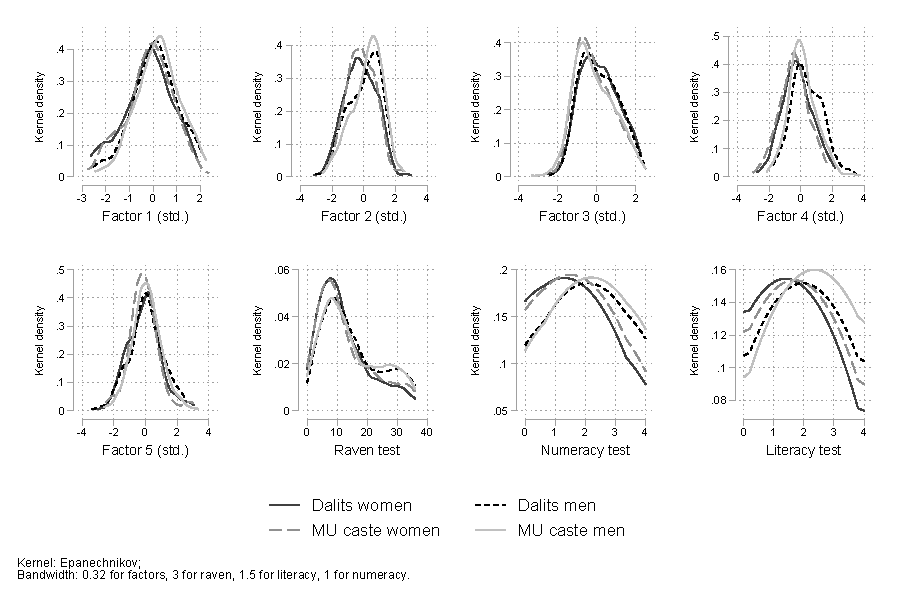
\includegraphics[width=\textwidth]{INPUT/Kernel_perso}
\caption{Distribution of cognitive skills and personality traits -- The resulting cognitive score and personality trait is based on the standardised residual from univariate OLS regression with age as exogenous variable. This is the cognitive score and personality trait purged from life-cycle effects}
\sourcefig{NEEMSIS (2016-17); author's calculations.}
\label{fig:EGOscore}
\end{figure}



\paragraph{Individual debt with Table \ref{tab:descY} and \ref{tab:descXY}}

Dalits female are more indebted than others, but there is no statistical evidence: 79\% of dalits female while 71\% for others.
Middle-upper caste male have highest total loan amount (124,440 INR that represent 1.21 years of labour income for the average dalit male), relatively similar for other groups (mean around 66,000 INR).
But, the distribution is very different: median at 54 for dalits female, around 24 for dalits male and non-dalits female.

Number of loans 

IDSR, share of income for principal and interest repayment can represent the burden of debt: double jeopardy for dalits female 185.87\% on average and 44\% for 50\% of individuals while 4\% for dalit male, 26\% for middle-upper caste female and 4\% for middle-upper caste male.


Female more over-indebted than male :


\subimport{INPUT}{desc_Y.tex}

Table \ref{tab:descXY} shows correlation test between personality traits \& cognitive skills and individual indebtedness measures.
For dalits, cognitive skills sems to be more correlated with debt than personality traits.
Indeed, Numeracy appears as well negatively correlated with indebtedness measure for dalits, as Raven.
Literacy seems to be positively correlated with individual debt for male while it is negatively correlated for female IDSR, whatever the caste.

Factor 1 --as Extraversion-Openness, is significantly positively correlated with individual debt service ratio for dalits female while, for dalits male, Factor 3 --as ESCO, is significantlty negatively correlated with the probability of being in debt in 2020-21.
For middle-upper caste female, Factor 1 is more correlated with the probability of being in debt than Raven test (respectively -0.18 and -0.13) 
Factor 1 to 4 are always negatively correlated with indebtedness measure for non-dalits female, going against cognitive skills for individual debt service ratio: Factor 3 and Factor 4 are negatively correlated while Raven, Numeracy and Literacy are positively correlated with the ratio.

Last, for non-dalits male, Factor 1 pulls debt in opposite directions depending on the measure used: it is positively correlated with loan amount and over-indebtedness (strongest relation with loan amount) and negatively correlated with the number of loans.
\dev{Peut-être car les gens très F1 ont peu de prêts mais des montants élevés, ca semble cohérent avec les hommes qui empruntent plus pour un besoin économique, donc besoin d'être EXOP alors que Femme petits prêts mais beaucoup : il n'y a que voir les montants avec les stat descriptives précédents}







\subimport{INPUT}{desc_XY.tex}







\newpage
% ***********************************
\section{Results}
% ***********************************
%As stated by \cite{Amrhein2019, Wasserstein2019, Wasserstein2016} reported confidence interval


\subimport{INPUT}{AME_indebt.tex}
\subimport{INPUT}{AME_loans.tex}
\subimport{INPUT}{AME_loanamount.tex}
\subimport{INPUT}{AME_IDSR.tex}
\subimport{INPUT}{AME_over40.tex}








%https://www.jwe.cc/2012/03/stata-latex-tables-estout/
% \begin{table}[htpb]
% \centering
% \begin{threeparttable}
% \caption{Total sample and first part of main variables}
% \label{econ:all_global_p1}
% \estauto{INPUT/econ_all_global_p1}{8}{S S S S S S S S}
% %\starnote
% \fignote{$\sym{*}~~p<0.10, \sym{**}~~~p<0.05, \sym{***}~~~~~p<0.01$. $\ssymbol{2}$ for 1,000 INR. $\ssymbol{3}$ Owner.}
% \sourcetab{RUME (2010) and NEEMSIS (2016-17); author's calculations.}
% \end{threeparttable}
% \end{table}	






\newpage
% ***********************************
\section*{Conclusion}
\addcontentsline{toc}{section}{Conclusion}
\label{Conclusion}
% ***********************************

Les programmes de MC qui essayent de cibler les plus pauvres ne sont pas super efficient car même chez eux, il y a beaucoup de situation différentes en termes de dette.
Pose la question de l'inclusion financière


\clearpage
\newpage
%-------------------------------------------------------------------------------%
%\begin{nolinenumbers}
\addcontentsline{toc}{section}{Références}
\bibliography{C:/Users/Arnaud/Dropbox/Arnaud/Ref_Arnaud}
%\nocite{*}



\newpage
%-------------------------------------------------------------------------------%
\appendix





% \numberwithin{table}{section}
% \numberwithin{figure}{section}

\section*{Appendix}
\label{app:APP}

\section{Data description}
\label{app:data}

In 2016-17, 492 households, 2,696 individuals, 953 egos.
But, 2 households without egos.
So we have 490 households and 953 egos.
NEEMSIS2 (2020-21) recovered 485 households, 2,635 individuals.
But, 600+1 individuals have left their households between the two wave, whose 98 egos.
Which mean that we have 485 housholds and 2,034 individuals.
But, we always have our two households without egos in 2016-17 that we can not compare.
Thus, we have 483 households.
But, for 10 households all egos have changed between 2016-17 and 2020-21.
Egos of 2016-17 are still here in 2020-21, but they do not be selected as egos. 
Finally, our sample is constitute from 835 egos represented 473 households.


\clearpage
\newpage
\section{Stability of Big-5 personality traits over time}
\label{section:stab_big5}

\begin{figure}[htpb]
\raggedright
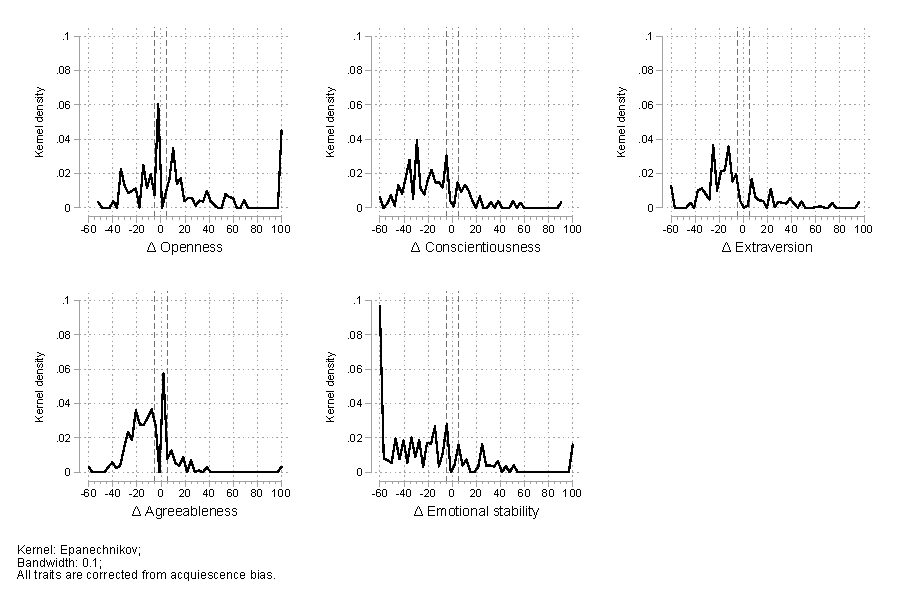
\includegraphics[width=\textwidth]{INPUT/Stabcorr}
\caption{Stability over time of Big-5 personality traits -- Distribution of variation rate between 2016-17 and 2020-21 for Big-5 personality traits corrected from acquiescence biais for 835 individuals from rural Tamil Nadu, India.}
\sourcefig{NEEMSIS-1 (2016-17) \& NEEMSIS-2 (2020-21); author's calculations.}
\label{fig:stab}
\end{figure}



\clearpage
\newpage
\section{Factor analysis for personality traits}
\label{section:efa_big5}

\subimport{INPUT}{Factor1.tex}
\subimport{INPUT}{Factor2.tex}
\subimport{INPUT}{Factor3.tex}
\subimport{INPUT}{Factor4.tex}
\subimport{INPUT}{Factor5.tex}

\subimport{INPUT}{Stdfactor.tex}

\subimport{INPUT}{anova_perso.tex}






\clearpage
\newpage
%-------------------------------------------------------------------------------%
\setcounter{tocdepth}5
\tableofcontents

%\end{nolinenumbers}
\end{document}


% % ***********************************
% \subsection{Hypothesis}
% % ***********************************

% As we already note, the goal of this paper is to analyze the role of cognitive skills and personality traits on indebtedness in a context where \jati and gender conditionned individuals.


% firstly, check the contextual determinants of debt.
% Then, we add personality traits \& cognitive skills in the analysis to answer our first question: is cognitive skills and personality traits plays a significant role on indebtedness situation of households in rural India?
% Following literature, we can make H\ref{hyp:stability}.
% Indeed, concerning conscientiousness, \cite{Donnelly2012} state that ``highly conscientious individuals manage their money more because they have positive financial attitudes as well as a future orientation''.
% \cite{Brown2014, Nyhus2001} find similar results: conscientious individuals are less likely to have ever been in debt and conscientiousness is negatively related to the amount of unsecured debt.
% \cite{Nga2013} find that conscientiousness have a significant influence on risk aversion in Malaysia.
% \cite{Forlicz2019} find that for most of these countries there existed significant differences between debtors and debt-free individuals regarding the level of conscientiousness
% For neuroticism, \cite{Pinjisakikool2017b} find that emotional stability (inverse of neuroticism) significantly predict financial risk tolerance.

% \begin{hyp}[H\ref{hyp:stability}] \label{hyp:stability}
% Conscientiousness and neuroticism play significant role on household indebtedness [and over-indebtedness].
% \end{hyp}

% To understand the phenomenon more in depth, we decompose the analysis by caste, class and gender.
% The notion of class allow us to encompass ``property, wealth, occupation, income, and education'' \citep{Beteille2007}.
% We implement a multiple correspondance analysis with land property, wealth, occupation and income\footnote{We choose to not take into account education to stay at household level.} to create a dichotomy between high and low class (see appendix \ref{section:mca_class}).
% For caste and class decomposition, we formulate H\ref{hyp:poorer} imagining that cognitive skills are more important for lower households because we can imagine that higher one have all a high level of cognitive skills (math, literacy, etc.) because of better level of education\footnote{For the link between caste and education, see \cite{Borooah2005}.}.
% %\cite{Gaurav2012} find that cognitive skills significantly predict the financial aptitude and debt literacy for rural farmer in Gujarat
% %\cite{Agarwal2013} finds that ``consumers with higher math scores, are substantially less likely to make a financial mistake'' in separating our sample between economically and socially upper households and economically and socially lower households.
% \begin{hyp}[H\ref{hyp:poorer}] \label{hyp:poorer}
% Cognitive skills are better predictors for lower households than for higher one. 
% \end{hyp}

% Concerning gender, as \cite{Reboul2020} stated: ``[w]omen in the poorest households, despite meager incomes, have the highest borrowing responsibilities, shouldering the highest shares of household debt. [...] Their larger role in household debt management may be linked to their greater mobility and lower restrictions on social interactions, notably with men, which would underpin both their greater income shares and their access to credit relations. ''
% Thus, we can formulate the H\ref{hyp:women} hypothesis.
% \begin{hyp}[H\ref{hyp:women}] \label{hyp:women}
% When ego is a woman, her cognitive skills and personality traits play a bigger role in household finances than when ego is a man.
% \end{hyp}

% \cite{Reboul2019} Far beyond the issue of information about wages, the management of family finances leads
% to constant tensions and conflicts among family members, and thus gives rise to various tactics
% aimed at partially overcoming family constraints. This is particularly true for women, who have
% a heavy responsibility to ensure, among other things, daily expenses


% Last, we explore the source and use of debt in creating the dichotomy formal--informal and income generator--non-income generator of debt.
% Following results of \cite{Brown2014}, we formulate H\ref{hyp:filr}.
% \begin{hyp}[H\ref{hyp:filr}] \label{hyp:filr}
% Conscientiousness, extraversion, agreeableness and openess to experience have an association with informal debt.
% \end{hyp}

% To try to verify our hypotheses, we use original data set from rural south India.

% \cite{Guerin2014a} il faut aussi que je regarde le rôle des compétences cognitives sur la négociation de la dette en cross section : qui sont ceux qui arrivent le mieux à négocier leur dette ? 
% Comment savoir la negociation de la dette ? C'est le prix de la dette
% Prix de la dette p16 de \cite{Guerin2014a} The cost of \textit{terinjavanga} loans








% % ***********************************
% \section{Pistes en réflexions}
% % ***********************************

% \begin{itemize}[label=--]
% \item Quel est le score de l'\textit{homo oeconomicus} en termes de \textit{Big Five} ? \citep{Lopez2020}
% \item À partir de là, on peut chercher à voir si les autoentrepreneurs sont des \textit{homo oeconomicus} ou s'ils sont \textit{schumpeterien} ou \textit{coasien}.
% \item Analyse \textit{schumpeterienne} : \url{https://doi.org/10.4000/interventionseconomiques.1481}
% \item Regarder les articles de \cite{Gong2020} et de \cite{Srinivasan2005}
% \item Voir Occupational Attainment and Earnings in Southeast Asia: The Role of Non-cognitive Skills de Labour Economics, 2020
% \item salaire (y) = perso (x) -> OK; salaire (y) = perso (x) + educ (x) -> pas OK; perso passe par educ
% \item soulèvent; pointent; surlignent; mettent en évidence
% \item \cite{Yilmazer2005} + \cite{Poterba2001} + \cite{King1982}
% \end{itemize}





%---------------------------------
%KEEP THAT BUT NOT IN THE ARTICLE
%---------------------------------
%\paragraph{Retirement assets}
%Compared to China, the retirement pensions are not very efficient.
%Indeed, around 90\% of labor is informal [in the sense of absence of social insurance] and 85\% of non-agricultural workforce is informal \citep{Mehrotra2019}.
%For \cite{Badarinza2016b}, India figures as an outlier among low-middle-income countries on this point.
%\paragraph{Gold}
%\begin{itemize}
%\item On average, gold represent more than 11\% of indien household balance sheet  while it is less than 1\% in China \citep{Badarinza2016b}.
%\item Préciser les différences rurales urbaines de \cite{Badarinza2016b}.
%\item Mais rester sur le fait qu'au TN l'or est la première forme d'épargne d'après \cite{Roesch2008} \cite{Guerin2012a}
%\item Pourquoi ils aiment tant ?
%\item[1] Real estate has lower liquidity when compared with gold, and if liquidity needs are correlated with inflation volatility, gold better serves the purpose than real estate. Gold as a non-financial asset also has additional properties that are not provided for by real estate, such as a high collateral value and physical verifiability \citep{Badarinza2016b}
%\item[2] Avec la littérature d'Isabelle, parler du social role de l'or en rural India.
%\end{itemize}
%---------------------------------






% Mesure overindebtedness
% \item \citep{European2010} ont 5 recommendations pour bien mesurer:
% \item[1] Le surendettement s’analyse au niveau du ménage car les revenus des individus sont généralement regroupés ;
% \item[2] Les indicateurs doivent couvrir tous les aspects des engagements financiers : le logement, le crédit à la consommation, les factures, les emprunts hypothécaires ;
% \item[3] Le surendettement est considéré comme un état structurel car il implique une incapacité à faire face à des dépenses récurrentes ;
% \item[4] Le surendettement ne se résout pas en empruntant davantage ;
% \item[5] Pour qu’un ménage respecte ses engagements, il doit réduire considérablement ses dépenses ou trouver un moyen d’accroître ses revenus.




%\cite{John1999} the Big 5 "represent personality at the broadest level of abstraction, and each dimension summarizes a large number of distinct, more specific personality characteristics".